% !TEX root = ./report.tex

\clearpage
\section{Background}
\label{background}

\subsection{The Regionalized Value-State Dependence Graph}
\label{background:RVSDG}

The \textit{Regionalized Value-State Dependence Graph} (RVSDG) is a
\textit{directed acyclic graph} (DAG) and a \textit{demand-based dependence
graph} (DDG), consisting of nodes representing computations and edges
representing the dependencies between nodes. Each node has inputs and outputs
connected through edges. The arity and order of inputs and outputs depend on the
operation the node represents, and they also needs to have the same arity and
order across all nodes representing the same operation.

In this report, we will discuss two kinds of nodes, and two kinds of edges: the
simple- and complex- nodes, and the data- and state- dependency edges. Simple
nodes represent the ``basic operations'', such as addition and subtraction.
Complex nodes contain another RVSDG subgraph, also called \textit{regions}. The
Complex nodes presented in this section are the $\gamma$-, $\theta$-,
$\lambda$-, and $\phi$-nodes.

\subsubsection{Edges}

The RVSDG has two types of edges: the data dependence edge, and the state
dependence edge, which represent the data and state values (respectively) of the
edges. The data dependence edge represents a data dependency one node has to
another, producing the value for the next computation.

State dependence edges preserve the semantics of the original program, keeping
the ordering of the nodes consistent with the program's flow of execution.
Stippled lines are used to denote state dependence edges in the figures of this
report. An example is shown in Figure~\ref{fig:for_loop_rec_fib_print_ex}.

\subsubsection{Nodes}

Of the two previously mentioned categories of nodes, simple nodes are used in an
RVSDG to represent simple operations, such as addition and subtraction.

A special case of the simple nodes listed in this report is the
\textit{apply}-node, which always has an edge linking a $\phi$-region or
$\lambda$-node as first input. The arity and order of the rest of the
\textit{apply}-node's inputs must match the order and arity of the inputs for
the $\lambda$-node linked directly or through a $\phi$-region. While a
$\phi$-region or $\lambda$-node may each link to duplicate \textit{apply}-nodes
representing the same function call, an \textit{apply}-node can (and must)
always one $\phi$-region or $\lambda$-node.

The complex nodes of an RVSDG relevant for an inliner are as follows:

\begin{itemize}

\item \textbf{$\gamma$-nodes: N-way statements}

\textit{$\gamma$}-nodes represent conditional statements. Each $\gamma$-node has
a predicate as input. All other edges passing into the $\gamma$-node are edges
its subsection's subgraph(s) depend upon. All subsections must have the same
order and arity of inputs and outputs, even if the subgraph in each case does
not depend on all of the inputs, or modify all of the outputs.

A $\gamma$-node most closely represents a \textit{switch-case} without fall-
through in each case. Each case of the switch statement corresponds then with a
subsection of the $\gamma$-node.

Hence, a simple \textit{if-statement} with no else-clause can be represented by
a $\gamma$-node with two subsections. The true subsection containing the RVSDG
subgraph representing the body of the if-statement. The false subsection of the
$\gamma$-node simply routing through all inputs straight out again unmodified.

How nested $\gamma$-nodes can represent the semantics of \textit{if, else if,
else} is shown in Figure~\ref{fig:nested_ifs}.

\begin{centering}
	\noindent\begin{minipage}{0.36\textwidth}
		\begin{lstlisting}[label={lst:nested_ifs}, style=customcpp]
if(smth){
	//do something 1
} else if(smth2){
	//do something 2
} else{
	//do something else
}
		\end{lstlisting}
	\end{minipage}
	\noindent\begin{minipage}{0.55\textwidth}
		\captionsetup{type=figure}
		\includegraphics[width=\textwidth]{figures/if_elseif_else_example}
	\end{minipage}
	\captionof{figure}{Minimal example of two nested $\gamma$-nodes representing
the the same semantics as the C/C++ pseudo code on the left.}
	\label{fig:nested_ifs}
\end{centering}

\item \textbf{$\theta$-nodes: Tail-controlled loops}

\textit{$\theta$}-nodes represent tail controlled loops. Like with the
$\gamma$-node, its input is the predicate. All other edges are the dependencies
needed by its subgraph(s) representing the statements in the body of the loop.

In C/C++ $\theta$-nodes are equivalent to \textit{do-while loops} containing the
subgraph representing of the body of the loop inside the node. Other loops, such
as \textit{for-loops}, can be represented by putting a $\theta$-node inside of
the \textit{true} clause of a $\gamma$-node with no subgraph in the subsection
of the \textit{false} clause. The $\gamma$- and $\theta$-nodes both need to have
the exact same predicate, and same dependencies on the predicate, if the
combined subgraph is to represent a for-loop.

See Figure~\ref{fig:for_loop_rec_fib_print_ex} for an example of a $\theta$-node
with corresponding C/C++ code in Listing~\ref{lst:for_loop_rec_fib_print_ex}.
The stippled directed edges in Figure~\ref{fig:for_loob_rec_fib_print_ex} denote
state dependencies between nodes.

\begin{lstlisting}[label={lst:for_loop_rec_fib_print_ex}, style=customcpp,
caption={C/C++ code corresponding to the RVSDG subgraph in
Figure~\ref{fig:for_loop_rec_fib_print_ex}.}]
for(int i = 0; i < 7; ++i){
	std::cout << "Fib #" << i << ": " << recursive_fibonacci(i) << std::endl;
}
\end{lstlisting}
\vspace{-4\parskip} %http://tex.stackexchange.com/q/40863
\newpage

\begin{figure}[ht!]
	\centering
	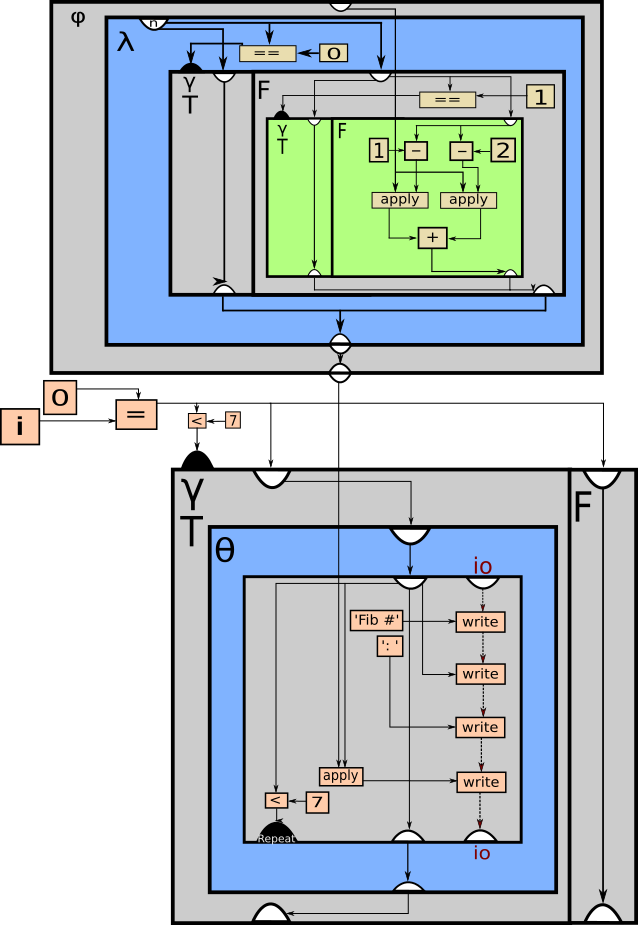
\includegraphics[width=\textwidth]{figures/for-loop-printf-rec_fib-example}
	\caption{A program consisting of a $\theta$-node looping 7 iterations,
calculating and printing the 7 first Fibonacci numbers. The $\theta$-node's
apply-node uses the same recursive Fibonacci function as in
Figure~\ref{fig:rec_fib_phi}.}
	\label{fig:for_loop_rec_fib_print_ex}
\end{figure}

\clearpage
\item \textbf{$\lambda$- and \textit{apply}-nodes: Functions}

\textit{$\lambda$}-nodes represent functions, and these are paired with at least
one \textit{apply}-node. Their \textit{apply}-nodes represent the call sites of
the function. There is only one $\lambda$-node per function in the program the
RVSDG represents. All \textit{apply}-nodes have an edge linking it to its
corresponding $\lambda$-node.

As with the other complex nodes, the order and arity of inputs needed for the
subgraph of the $\lambda$-node need to match the order and arity of the inputs
and edges in its corresponding \textit{apply}-nodes.

The \textit{apply}-nodes however, have an extra first input, the edge linking
the corresponding $\lambda$-node to the \textit{apply}-node. Except for when the
$\lambda$-node is in a $\phi$-region, there are no edges into a $\lambda$-node,
only into \textit{apply}-nodes. Conversely, the only edges going out of
$\lambda$-nodes when it's outside of a $\phi$-region, are the edges which each
link to an \textit{apply}-node representing a call sites for the function.

\item \textbf{$\phi$-regions: Recursive environments}

\textit{$\phi$}-regions represent parts of the program's semantics where
functions behave recursively. They behave recursively either by calling
themselves (regular recursion), or two or more calling each other and making a
recursive tree or containing at least one cycle (mutually recursive).

To uphold the DAG properties of an RVSDG, the RVSDGs containing a $\phi$-region
solve this by encasing the recursive/mutually recursive function(s), in a
$\phi$-region. A $\phi$-region has, like the $\lambda$-nodes, no inputs, but an
output for each function contained within.

The recursion's implicit cycle is solved by having the link going from
$\lambda$-nodes to  \textit{apply}-nodes go from the top of the $\phi$-region
and down to each apply node contained in the subgraph within. The order and
arity of the ``outputs'' going out from the top inside of the $\phi$-region and
to each \textit{apply}-node, has to match the order and arity of the outputs for
each function on the ``bottom'' and outside of the $\phi$-region.

Figure~\ref{fig:rec_fib_phi} illustrates how a $\phi$-node containing the
representation of a recursive fibonacci function would look like in an RVSDG.

\end{itemize}

\todo[inline]{Fix Figure~\ref{fig:rec_fib_phi}...}

\begin{figure}[h!]
	\centering
	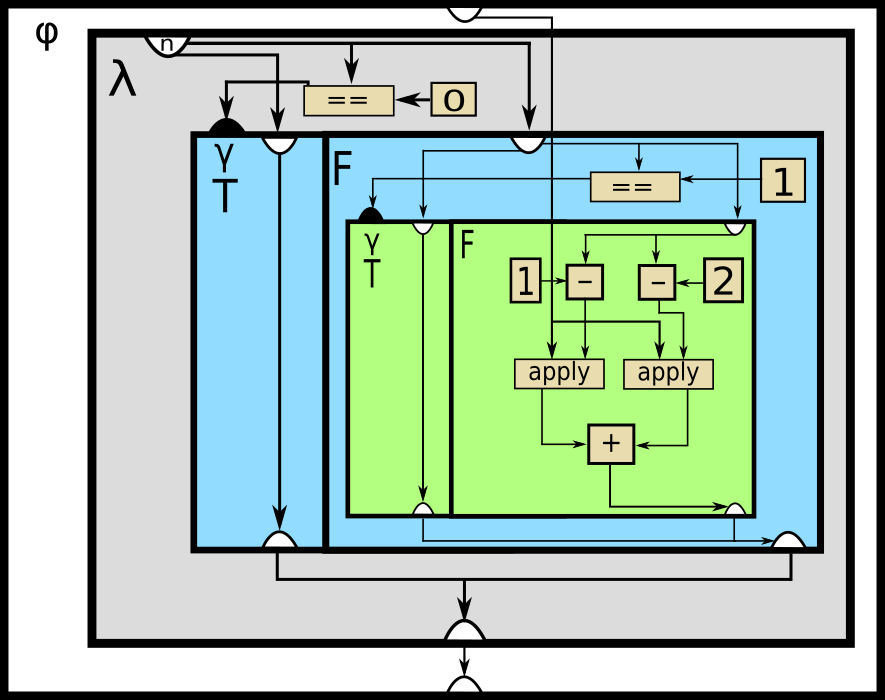
\includegraphics[width=0.75\textwidth]{figures/recursive_fibonacci}
	\caption{A $\phi$-node containing a $\lambda$-node representing a recursive
version of a function producing the $n$ first numbers in the Fibonacci series.}
	\label{fig:rec_fib_phi}
\end{figure}
